\section{Optimal Control of Pitch/Travel without Feedback}\label{sec:prob2}

\subsection{State space form}\label{sec:prob21}
For Problem 2 an optimal control sequence had to be calculated disregarding the elevation \emph{e} and relinquishing feedback. The states were given by the problem description with $\mathbf{x}= \begin{bmatrix} \lambda & r & p & \dot p \end{bmatrix}^\top$ and the only input was given by $u = p_c$. Therefore the model can be written in time state space form in the following way: 
\begin{equation} \label{statespace2}
	\underbrace{\begin{bmatrix}
		\dot \lambda \\
		\dot r \\
		\dot p \\
		\ddot p
	\end{bmatrix}}_\text{$\mathbf{\dot x}$}
	=
	\underbrace{\begin{bmatrix}	
				0 & 1 & 0 & 0 \\
				0 & 0 & -K_2	& 0 \\
				0 & 0 & 0 & 1 \\
				0 & 0 & -K_1K_{pp} & -K_1K_{pd}
	\end{bmatrix}}_\text{$\mathbf{A_c}$}
	\underbrace{\begin{bmatrix}
		\lambda \\
		r \\
		p \\
		\dot p
	\end{bmatrix}}_\text{$\mathbf{x}$}
	+
	\underbrace{\begin {bmatrix}	
				0 \\
				0 \\
				0 \\
				K_1K_{pp}			
	\end{bmatrix}}_\text{$\mathbf{B_c}$}
	\underbrace{
		\vphantom { 
			\begin {bmatrix}	
				0 \\
				0 \\
				0 \\
				K_1K_{pp}			
			\end{bmatrix}
		}
		p_c
	}_\text{u}
\end{equation}

\subsection{Discussion of the model}\label{sec:prob22}
The control hierarchy of the model is displayed in following figure:
\begin{figure}[h]
	\centering
	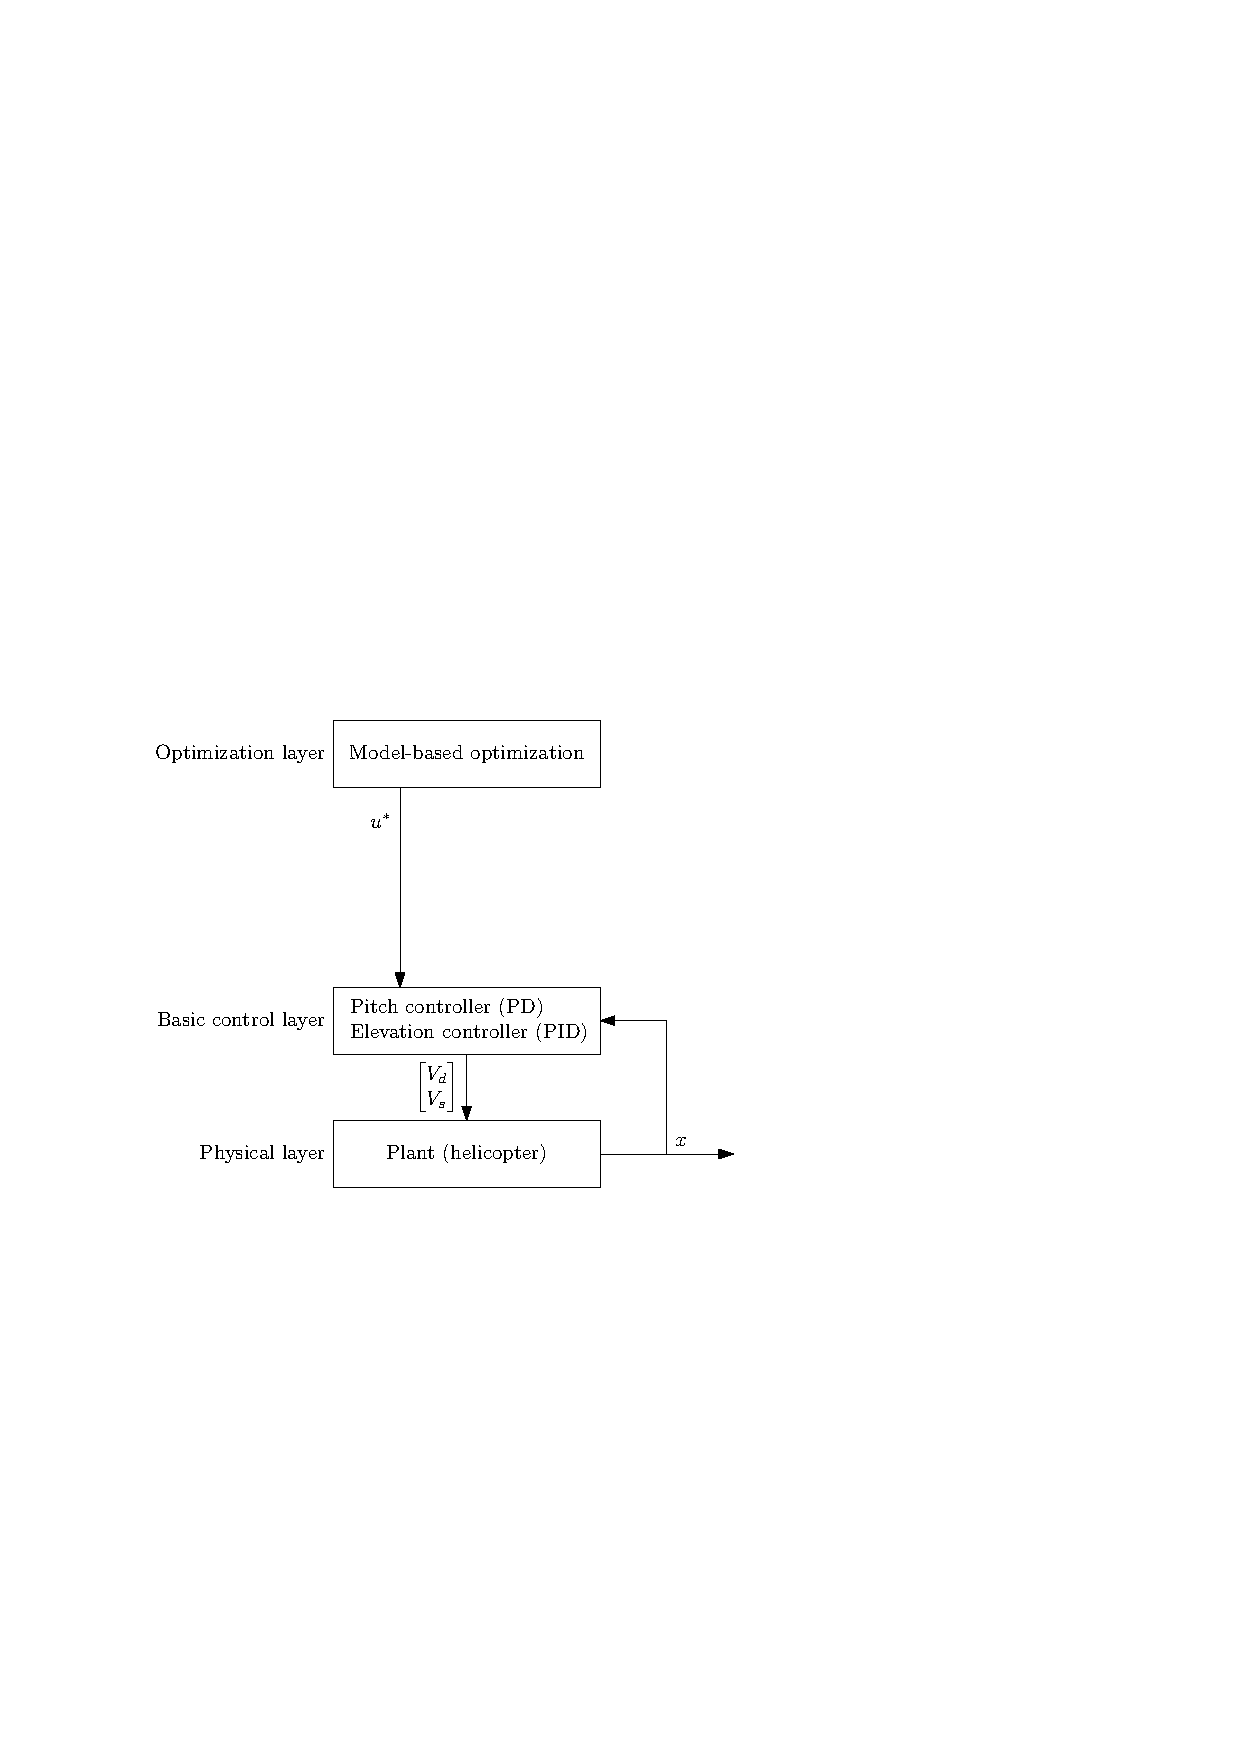
\includegraphics[width=1.0\textwidth]{figures/layers_openloop.pdf}
	\caption[Control hierarchy as used in Problem 2]{Control hierarchy\footnotemark as used in Problem 2}
	\label{fig:layers_openloop}
\end{figure}
\footnotetext {as depicted in the problem description}
\newline
Since the model as presented above also contains the pitch and elevation setpoints as inputs it does not only depict the phyiscal behaviour of the helicopter. Instead also the inner control loops of pitch and elevation are modeled.
\subsection{Discretisation}\label{sec:prob23}
In order to use the time state space form to calculate the optimal trajectory from the optimal control sequence it had to be discretised in time. For the discretisation the forward Euler method was used:
\begin{equation}
	\mathbf{x_{k+1}}= \mathbf{x_k}+ \Delta t \mathbf{\dot x_k}
\end{equation}
using the time state space form (\ref{statespace2})
\begin{align}
	\mathbf{x_{k+1}}&=\mathbf{x_k+ (A_cx_k+B_c}u_k) \Delta t \nonumber \\ 
			&=(\mathbf{I} + \Delta t\mathbf{ A_c})\mathbf{x_k}+\Delta t \mathbf{B_c}u_k \nonumber \\
			&=\mathbf{Ax_k+B}u_k
\end{align}
\begin{equation}
	\mathbf{A} =
	\begin{bmatrix}
				1 & \Delta t & 0 & 0 \\
				0 & 1 & -K_2\Delta t& 0 \\
				0 & 0 & 1 & \Delta t \\
				0 & 0 & -K_1K_{pp}\Delta t & 1-K_1K_{pd}\Delta t
	\end{bmatrix}, \quad
	\mathbf{B} =
	\begin{bmatrix}	
				0 \\
				0 \\
				0 \\
				K_1K_{pp}\Delta t			
	\end{bmatrix}
\end{equation}
For the discretisation a time step $\Delta t = 0.25 \mathrm{s}$ was used.

\subsection{Optimal trajectory}\label{sec:prob24}
For the starting point $\mathbf{x_0} = \begin{bmatrix} \lambda_0&0&0&0\end{bmatrix}^\top$ and the terminal point $\mathbf{x_f}=  \begin{bmatrix} \lambda_f&0&0&0\end{bmatrix}^\top$ the optimal trajectory had to be calculated. $\lambda_0$ was set to $\pi$ and $\lambda_f$ was set to $0$.So the helicopter should make a curve of 180\textdegree and then remain at his position. In order to find the optimal trajectory the following cost function was minimised with different weightings $q$ for the pitch input $p_{ci}$:
\begin{equation}
\phi = \displaystyle\sum_{i=1}^{N} (\lambda_i-\lambda_f)^2+qp_{ci}^2, \quad q \geq 0
\end{equation}
Additionally the following constraint on the input value was implemented:
\begin{equation}
	|p_k|\leq \frac {30\pi} {180}, \quad k \in \{1, \dots,N\}
\end{equation}
The constraint prevents the helicopter from flying rather extreme manoeuvres where the pitch angle exceeds 30\textdegree and thus contributes to the overall safety of the equipment and the laboratory staff. Since the cost function is quadratic in both variables, the pitch input and the deviation of the position from the terminal point, it can be solved by quadratic programming algorithms. Though the helicopters position will always be compared to the terminal point. This may result in fast helicopter movement and aggressive steering, which can be hard to handle due to the helicopter's momentum. High pitch angles may also exceed the area in which the system equation are sufficiently accurate since they rely on small angle approximations. Also aggressive inputs on the pitch control may cause the pitch angle to exceed the constraints due to the momentum of the helicopter.
\subsection{Results of the optimization}\label{sec:prob25}
To solve the optimization problem the $\mathrm{MATLAB}$ function \texttt{quadprog} was used. Values of 0.1, 1, and 10 were chosen for the weighting factor $q$. 5 seconds of zeroes were added before and after the control sequence in order to give the helicopter some time to stabilise. The results were exported from $\mathrm{MATLAB}$ and are depicted in the Figures (\ref{fig:problem2plots_q_1.0}),  (\ref{fig:problem2plots_q_0.1}) and  (\ref{fig:problem2plots_q_10}).
\begin{figure}[h]
	\centering
	\ProblemTwoPlot{../MATLAB/Export/problem2plots_q_1.0.csv}{../MATLAB/Export/problem2plots_q_1.0_opt.csv}
	\caption{Results for $R=1.0$}
	\label{fig:problem2plots_q_1.0}
\end{figure}

\begin{figure}[h]
	\centering
	\ProblemTwoPlot{../MATLAB/Export/problem2plots_q_0.1.csv}{../MATLAB/Export/problem2plots_q_0.1_opt.csv}
	\caption{Results for $R=0.1$}
	\label{fig:problem2plots_q_0.1}
\end{figure}

\begin{figure}[h]
	\centering
	\ProblemTwoPlot{../MATLAB/Export/problem2plots_q_10.csv}{../MATLAB/Export/problem2plots_q_10_opt.csv}
	\caption{Results for $R=10$}
	\label{fig:problem2plots_q_10}
\end{figure}

As expected a lower value for $q$ allows much stronger inputs than higher values. This is logical since a higher value for $q$ emphasizes the influence of the inputs in the cost function. Therefore the higher $q$ is the less inputs are given in order to keep the value of the cost function low. Still, regardless of the value of $q$ the helicopter does not remain at his terminal point but continues moving as we can see in the plot of $\lambda$. This behaviour can be ascribed to the missing feedback. The helicopter does only follow the control sequence that has been calculated in advance and does not compare the setpoints with his current state. 



